\section{Formula Sheet}
\subsection{Basics}
\paragraph{Standard Deviation} $$SD(x) = \sqrt{\frac{1}{n-1}\Sigma_i (x_i - \bar{x})^2}$$
\paragraph{Variance} $$Var(x) = \frac{1}{n-1}\Sigma_i (x_i - \bar{x})^2$$
\paragraph{Covariance} $$Cov(x,y) = \frac{1}{n-1}\Sigma_i (x_i - \bar{x})(y_i - \bar{y})$$
\paragraph{Normal Distribution} $$f(x) = \frac{1}{\sigma \sqrt{2\pi}}e^{-\frac{(x-\mu)^2}{2\sigma^2}}$$
standardized: $$Z = \frac{X - \mu}{\sigma}$$
\paragraph{Probability density function (pdf): f(x)} $$f(x) = P(X = x)$$

\paragraph{Cumulative distribution fuction (cdf): F(x)} $$F(x) = P(X \leq x)$$ $$P(X \geq x) = 1 - F(x)$$  $$P(x_1 \leq X \leq x_2) = F(x_2) - F(x_1)$$
\paragraph{Confidence Interval} $$CI = \left[ \bar{X} - z_{(1 - \frac{\alpha}{2})}\cdot \frac{\sigma}{\sqrt{n}} , \bar{X} + z_{(1 - \frac{\alpha}{2})}\cdot \frac{\sigma}{\sqrt{n}} \right] $$
$$CI = \left[ \bar{X} - t_{(1 - \frac{\alpha}{2})}\cdot \frac{s}{\sqrt{n}} , \bar{X} + t_{(1 - \frac{\alpha}{2})}\cdot \frac{s}{\sqrt{n}} \right] $$
\subsection{Linear Regression}
\subsubsection{First Order Linear Model}

$$Y = \beta_0 + \beta_1 X + \varepsilon$$

\paragraph{OLS Estimator}

\begin{align*}
	\hat{\beta}_1 &= \dfrac{\frac{1}{n-1}\Sigma_i (x_i - \bar{x})(y_i - \bar{y})}{\frac{1}{n-1}\Sigma_i (x_i - \bar{x})^2} = \frac{Cov(x,y)}{Var(x)} \\ \ \\
	\hat{\beta}_0 &= \bar{y} - \hat{\beta}_1\cdot \bar{x} \\ \ \\
	\hat{y} &= \hat{\beta}_0 + \hat{\beta}_1 x
\end{align*}	

\subsubsection{Multiple Linear Regression Model}
$$Y = \beta_0 + \beta_1 X_1 + \beta_2 X_2 + \dots + \beta_k X_k + \varepsilon$$
Formulation in \textbf{matrix form}:
$$\begin{bmatrix}
y_1 \\ y_2 \\ \vdots \\ y_m
\end{bmatrix} = \begin{bmatrix}
1 & X_11 &X_12 &\dots &X_1k \\
1 & X_21 &X_22 &\dots &X_2k \\
\vdots & \vdots &\vdots &\vdots &\vdots \\
1 & X_m1 &X_m2 &\dots &X_mk
\end{bmatrix} \begin{bmatrix}
\beta_0 \\ \beta_1 \\ \beta_2 \\ \vdots \\ \beta_k
\end{bmatrix} + \begin{bmatrix}
\varepsilon_1 \\ \varepsilon_2 \\ \vdots \\ \varepsilon_m
\end{bmatrix}$$
$$[m \times 1] = [m \times (k+1)] \cdot [(k+1) \times 1] + [m \times 1]$$

\paragraph{OLS Estimator} 
\begin{itemize}
	\item Model:
	\begin{align*}
		RSS  &= e^{T} e = (y - X\hat{\beta})^T (y - X\hat{\beta}) \rightarrow \min \\
		\rightarrow  &\frac{\partial RSS}{\partial \beta} = -2X^Ty + 2X^TX\beta= 0
	\end{align*}
	
	\item Solution:
	\begin{align*}
		\hat{\beta} &= (X^TX)^{-1}X^Ty \\ 
		\hat{y} &= X(X^TX)^{-1}X^Ty
	\end{align*}

	


\end{itemize}
\subsubsection{Quality Metrics of Linear Regression Models}
\paragraph{Residual Sum of Squares (RSS)}
An \textbf{unbiased} estimator of RSS of the population is given by 
$$RSS = \Sigma_{i=1}^{n} (y_i - \hat{y}_i)^2$$

\paragraph{Mean Squared Error (MSE)}
$$MSE = \frac{RSS}{N}$$
\paragraph{Root Mean Squared Error (RMSE)}
$$RMSE = \sqrt{MSE}$$
\paragraph{Total Sum of Squares (TSS)} sum of Explained Sum of Squares(ESS) and Residual Sum of Squares(RSS).
\begin{align*}
	\Sigma (y - \bar{y})^2 &= \Sigma (\hat{y} - \bar{y})^2 + \Sigma (y - \hat{y})^2 \\
	TSS &= ESS + RSS
\end{align*}
\paragraph{R-squared $\mathbf{R^2}$} the proportional of explained variablity from the model
$$R^2 = \frac{TSS - RSS}{TSS} = 1 - \frac{RSS}{TSS} = \frac{ESS}{TSS}$$ 


\subsection{Logistic Regression \& Poisson Regression}
\subsubsection{The Logistic Regression Model}
The \textbf{binary} logistic regression model described in \textbf{log odds/logit}:
$$log\_odds  =  \ln(\frac{p(X)}{1 - p(X)}), \quad  \ln(\frac{p(X)}{1 - p(X)}) = \beta_0 + \beta_1 X + \varepsilon$$

The logistic regression model described in \textbf{odds}: 
$$odds = \frac{p(X)}{1 - p(X)}, \quad \frac{p(X)}{1 - p(X)} = e^{\beta_0 + \beta_1 X}$$

\subsubsection{The Logistic Function}
$$Pr[Y|X] = p(X) = \dfrac{e^{\beta_0 + \beta_1 X}}{1 + e^{\beta_0 + \beta_1 X}}$$

\subsubsection{Multiple Logistic Regression Model}
$$\ln(\frac{p(X)}{1 - p(X)}) = \beta_0 + \beta_1 X_1 + \beta_2 X_2 + \dots + \beta_k X_k$$

The logistic function can also be described as a \textbf{sigmoid function} in form $S(x) = \frac{e^x}{1 + e^x} = \sigma(x)$
$$P(X) = \sigma(\beta_0 + \beta_1 X)$$
\subsubsection{The Likelihood Function and Maximum Likelihood Estimator}
\paragraph{likelihood function for Logistic Regression Model}
\begin{align*}
	L &= \Pi_{i=1} p^{y_i}(1-p)^{1-y_i} \\
	&= \Pi_{i=1} \sigma(\beta_0 + \beta_1 X)^{y_i} \cdot (1 - \sigma(\beta_0 + \beta_1 X))^{1-y_i}
\end{align*}
\paragraph{Log of Likelihood Function}
$$LL = \ln(L) = \Sigma_{i=1} ( y_{i} \ln(p) + (1 - y_i)\ln(1-p))$$
\paragraph{Maximum Likelihood Estimator}
\begin{align*}
	\beta = \arg\max_{\beta}(LL) &= \arg\max_{\beta} [\Sigma_{i=1} ( y_{i} \ln(p) + (1 - y_i)\ln(1-p))] \\
	&= \arg\max_{\beta} [\Sigma_{i=1} ( y_{i} \ln(\sigma(\beta_0+\beta_1X)) + (1 - y_i)\ln(1-\sigma(\beta_0 + \beta_1X)))]
\end{align*}

\paragraph{Gradient(partial derivatives) of the LL-Function}: \textbf{chain rule}

with $z = \beta_0+\beta_1X$

$$\frac{\partial LL}{\beta_j} = \Sigma_{i=1} \frac{\partial LL}{\partial p} \cdot \frac{\partial p}{\partial z} \cdot \frac{\partial z}{\partial \beta_j}$$
\begin{align*}
	\frac{\partial LL}{\partial p} &= \frac{y_i}{p} - \frac{1 - y_i}{1 - p} \\
	\frac{\partial p}{\partial z} &= \sigma(z) \cdot(1 - \sigma(z)) \\
	\frac{\partial z}{\partial \beta_0} &= 1 \text{, } \frac{\partial z}{\partial \beta_j} = x_j\\		 
\end{align*}
\begin{align*}
	\frac{\partial LL}{\beta_0} &= \left[ \frac{y_i}{p} - \frac{1 - y_i}{1 - p}\right]  \sigma(z) \cdot(1 - \sigma(z)) = \left[ y_i - \sigma(X\beta) \right] \\
	\frac{\partial LL}{\beta_j} &= \left[ \frac{y_i}{p} - \frac{1 - y_i}{1 - p}\right]  \sigma(z) \cdot(1 - \sigma(z))\cdot x_j = \left[ y_i - \sigma(X\beta) \right] x_j
\end{align*}

\subsubsection{Poisson Regression Model}
$$ln(\mu(x)) = \beta_0 + \beta_1 X_1 + \dots \beta_j X_i$$

\paragraph{random component(dependent variable)}
$$Pr(Y|X) = p(X) = \dfrac{e^{-\mu} \mu^y}{y!} = \dfrac{e^{\beta xy} e^{-e^{\beta x}}}{y!}$$

\paragraph{likelihood function}
$$L(\beta|X,Y) = \Pi_{i=1} p = \Pi_{i=1} \dfrac{e^{\beta x_iy_i} e^{-e^{\beta x}}}{y_i!}$$

\paragraph{The Maximum Likelihood Estimator} 
$$\log L(\beta | X,Y) = \Sigma_{i=1} (\beta x_iy_i - e^{\beta x_i} - \log(y_i!))$$





\subsection{Naive Bayes \& Bayesian Network}
\subsubsection{Bayes Theorem}
\begin{itemize}
	\item single evidence: $$Pr(h|e) = \frac{Pr(h \cap e)}{Pr(e)} = \dfrac{Pr(e|h) \cdot Pr(h)}{Pr(e)}$$
	\item multiple evidence: 
	\begin{align*}
		Pr(h|e_1, e_2, \dots, e_k) &= \dfrac{Pr(e_1 | h) \cdot Pr(e_2 | h) \dots Pr(e_k | h) \cdot Pr(h)}{Pr(e_1, e_2, \dots, e_k)} \\ 
		&= \frac{\Pi_{i=1}^k Pr(e_i|h) \cdot Pr(h)}{Pr(e_1,e_2, \dots e_k)}
	\end{align*}
\end{itemize}

	
\subsubsection{Pr(e)}
\begin{itemize}
	\item If the prior probability $Pr(e_i)$ is \textbf{known}: 
	$$Pr(e_1, e_2, \dots, e_k) = Pr(e_1)\cdot Pr(e_2)\dots Pr(e_k)$$
	\item If the prior probability $Pr(e_i)$ is \textbf{unknown}: law of total probability
	$$Pr(e_1, e_2, \dots, e_k) = Pr(e_1, e_2, \dots, e_k|h)\cdot Pr(h) + Pr(e_1, e_2, \dots, e_k | \neg h) \cdot Pr(\neg h)$$
\end{itemize}

\subsubsection{Chain Rule}
According to the \textbf{directed acyclic graph}, derive the \textbf{joint probability distribution} 

$$Pr(e_1, e_2, \dots, e_k) = \Pi_{i=1} Pr(e_i| e_{i-1}, \dots, e_1) = \Pi_{i=1} Pr(e_i| \text{Parents}(e_i))$$

\subsubsection{Conditional Independence}
\paragraph{conditional independence between hypothesis and evidence} the hypothesis $h$ is only dependent on $e_1, e_2, e_3$, not on $e_4$ (redundant), then 
$$Pr(h | e_1, e_2, e_3, e_4) = Pr(h | e_1, e_2, e_3) $$

\paragraph{conditional independence between hypotheses}

if two hypotheses are \textbf{independent} from each other, then
$$Pr(h_1, h_2 | e_1, e_2) = Pr(h_1|e_1,e_2) \cdot Pr(h_2|e_1,e_2)$$











\subsection{Decision Tree}
\paragraph{Entropy} $\in [0,1]$, measures how much \textbf{additional information required} in \textbf{bits}
	$$\text{entropy}(p_1, \dots, p_n) = - \Sigma_{i=1} ^n p_i \cdot \log_{2} p_i$$
	
\paragraph{Information of Each Attribute Value}
	
	$$\text{info}([c_1, \dots, c_n]) = \text{entropy}(\frac{c_1}{C}, \dots, \frac{c_n}{C})$$ 
	
\paragraph{Information of the Attribute} the \textbf{weighted average} of the \textbf{information needed} from each attribute value. 

Say an attribute has $m$ attribute values/branches,

$$\text{info}([c_1, \dots, c_n]_1, \dots, [c_1, \dots, c_n]_m) = \Sigma_{i=1}^m  \frac{C_m}{N} \cdot \text{info}([c_1, \dots, c_n])_m$$

\paragraph{Information Gain of the Attribute} 

$$\text{Information\_Gain(attribute)} = \text{info(before split by attribute)} - \text{info(after split by attribute)}$$ 

\paragraph{Intrinsic Information of a Attribute} s: size of a leaf from each branch
$$\text{intrinsic\_info}([s_1, \dots, s_n]) = \text{info}([s_1, \dots, s_n])$$

\paragraph{Gain Ratio of a Attribute}

$$\text{Gain\_Ratio(attribute)} = \dfrac{\text{Gain(attribute)}}{\text{Intrinsic\_Info(attribute)}}$$


\subsection{Evaluation}

\paragraph{Accuracy} $$\text{Accuracy} = \frac{TP + TN}{N}$$
\paragraph{Error Rate} $$\text{Error Rate} = 1 - \text{Accuracy} = \frac{FP + FN}{N}$$

\paragraph{True Positive Rate / Recall / Hit Rate} $$\text{True Positive Rate/Recall} = \frac{TP}{TP + FN}$$
\paragraph{True Negative Rate / Specificity} $$\text{True Negative Rate/Specificity} = \frac{TN}{TN + FP}$$
\paragraph{False Positive Rate / False Alarm Rate} $$\text{False Positive Rate/False Alarm Rate} = 1- \text{Specificity} = \frac{FP}{TN + FP}$$

\paragraph{Precision} $$\text{Precision} = \frac{TP}{TP + FP}$$

\subsection{Clustering: Expectation Maximization}
\paragraph{Expectation Step} calculate the probability for \textbf{all instances} in \textbf{each cluster}.
$$Pr(A|x) = \frac{Pr(x|A) \cdot Pr(A)}{Pr(x)} ,\quad Pr(x|A) = \frac{1}{\sqrt{2\pi} \cdot \sigma_A} e^{-\frac{(x - \mu_A)^2}{2\sigma_A^2}}$$
$$Pr(B|x) = \frac{Pr(x|B) \cdot Pr(B)}{Pr(x)} ,\quad Pr(x|B) = \frac{1}{\sqrt{2\pi} \cdot \sigma_B} e^{-\frac{(x - \mu_B)^2}{2\sigma_B^2}}$$

\paragraph{Maximization Step} calculate the weighted mean and weighted variance using \textbf{all instances}. 
$$w_{iA} = Pr(A|x), \quad  w_{iB} = Pr(B|x)$$
$$\mu_A = \frac{w_{1A}x_1 + w_{2A}x_2 + \dots + w_{nA}x_n}{w_{1A} + w_{2A} + \dots + w_{nA}}$$
$$\sigma_A = \sqrt{\frac{w_{1A} (x_1 - \mu_A)^2 + \dots + w_{nA} (x_n - \mu_A)^2}{w_{1A} + w_{2A} + \dots + w_{nA}}}$$
analog to $\mu_B$ and $\sigma_B$

$$Pr(A) = \frac{\Sigma w_A}{\Sigma w_A + \Sigma w_B}, \quad Pr(B) = 1 - Pr(A)$$

\subsection{Principal Component Analysis \& Restoring Original Data}
\begin{figure}[H]
	\centering
	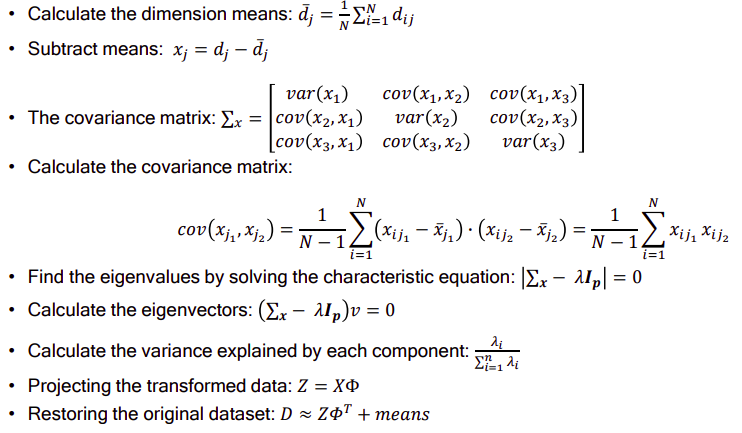
\includegraphics[width=\textwidth]{dimreduce.png}
\end{figure}
\newpage
\subsection{Recommendation Systems: Association Rules}
\paragraph{Support of a Rule}
\item support of \textbf{a rule}: the support of all item sets it contains. 
$$supp(A,B \Rightarrow C,D) = supp(\{A,B,C,D\})$$

\paragraph{Confidence of a Rule}  the probability that X and Y coexist given that X exists.
$$conf(R: X \Rightarrow Y) = \frac{supp(X \cup Y)}{supp(X)}$$

\paragraph{Lift of a Rule} indicates \textbf{by how much (ratio)} the \textbf{confidence of a rule} surpasses the \textbf{expected value}. 
$$Lift(R: X \Rightarrow Y) = \frac{conf(R)}{expConf(R)} = \dfrac{\frac{supp(X \cup Y)}{supp(X)}}{supp(Y)} = \frac{supp(X \cup Y)}{supp(X)\cdot supp(Y)}$$
\subsection{Recommendation Systems: Collaborative Filtering}
\paragraph{Weighted Correlation}
$$w_{a,u} = s_{a,u} \cdot c_{a,u}$$ 
$$c_{a,u} = \frac{Cov(r_{a}, r_{u})}{\sigma_{r_{a}} \cdot \sigma_{r_{u}}}$$
$$Cov(r_{a}, r_{u}) = \frac{1}{m-1}\cdot \Sigma (r_a - \bar{r}_a) (r_u - \bar{r}_u)$$

\paragraph{Rating Prediction}
$$p_{a,i} = \bar{r}_a + \Sigma_{u = 1}^k \dfrac{w_{a,u} \cdot (r_{u,i} - \bar{r}_u)}{\Sigma_{u=1}^k |w_{a,u}|}$$

\subsection{Recommendation Systems: SVD}
\paragraph{Rating Prediction}
$$r_{u,i} = \bar{r}_u + U(user) \cdot S \cdot V^T(item)$$


\subsection{Neural Network}
\paragraph{Forward Pass}
\begin{align*}
	z^{[1]} &= W^{[1]}\cdot a^{[0]} + b^{[1]} =  W^{[1]}\cdot x + b^{[1]}\\
	a^{[1]} &= g^{[1]}(z^{[1]}) = \sigma(z^{[1]}) \\
	z^{[2]} &= W^{[2]}\cdot a^{[1]} + b^{[2]} \\
	a^{[2]} &= g^{[2]}(z^{[2]}) = \sigma(z^{[2]})
\end{align*}

\paragraph{Loss Function} If we evaluate the model using \textbf{cross-entropy loss}: the calculation for $y \ln\hat{y}$ is a dot product(element-wise multiplication).
$$l(y,\hat{y}) = - [y \ln \hat{y} + (1-y)\ln(1 - \hat{y})]$$
\paragraph{Empirical Risk}  \textbf{average} the loss.
$$\mathcal{L}(y,\hat{y}) = \frac{1}{n} \cdot \Sigma l(y,\hat{y})$$

\paragraph{Backpropagation}

example in updating layer 2:
\begin{align*}
	W^{[2]}_{t+1} &= W^{[2]}_t - \alpha \cdot dW =W^{[2]}_t - \alpha \cdot \frac{\partial L}{\partial W^{[2]}} \\
	b^{[2]}_{t+1} &= b^{[2]}_t - \alpha \cdot db =b^{[2]}_t - \alpha \cdot \frac{\partial L}{\partial b^{[2]}} 
\end{align*}

	
$$\frac{\partial L_n}{\partial W} = \frac{\partial L_n}{\partial a_{n}} \cdot \frac{\partial a_{n}}{\partial z_{n}} \cdot \frac{\partial z_n}{\partial W}$$

\begin{align*}
	L_n &= \frac{1}{2} (y_{n} - g(w_{kl}a_{kn} + b_l))^2 = \frac{1}{2} (y_n - a_{ln})^2, \quad &\frac{\partial L_n}{\partial a_{ln}} &= -(y_n - a_{ln})\\
	a_{ln} &= g(z_{ln}) , \quad &\frac{\partial L_n}{\partial z_{ln}} &= g'(z_{ln}) \\
	z_{ln} &= w_{kl}a_{kn} + b_l, \quad &\frac{\partial L_n}{\partial w_{ln}} &= a_{kn} 	
\end{align*}

If the activation is a sigmoid activation: $\sigma(x) = \frac{e^x}{1 + e^x}$, $\sigma'(x) = \sigma(x)(1 - \sigma(x))$.
$$dW^{[2]} = -(y- a^{[2]})\cdot a^{[1]^{T}} = (a^{[2]} - y) \cdot a^{[1]^{T}}$$

\paragraph{Gradient Descent}

	\subparagraph{fixed step size}
	$$\begin{bmatrix}
	x_n \\y_n
	\end{bmatrix} = \begin{bmatrix}
	x_{n-1} \\ y_{n-1}
	\end{bmatrix} - \alpha \cdot \nabla f(x_{n-1}, y_{n-1})$$
	\subparagraph{dynamic step size}
	$$\begin{bmatrix}
	x_n \\y_n
	\end{bmatrix} = \begin{bmatrix}
	x_{n-1} \\ y_{n-1}
	\end{bmatrix} - \alpha_{n} \cdot \nabla f(x_{n-1}, y_{n-1})$$
	
	\subparagraph{Momentum}
	\begin{align*}
		d_n &= \beta \cdot d_{n-1} + \alpha \cdot\nabla f(x_{n-1})\\
		x_n &= x_{n-1} - d_n
	\end{align*}


